\documentclass{article}
\setlength{\parskip}{5pt} % esp. entre párrafos
\setlength{\parindent}{0pt} % esp. al inicio de un párrafo
\usepackage{amsmath} % mates
\usepackage{url} % que las URLs se vean lindos
\usepackage[top=25mm,left=20mm,right=20mm,bottom=25mm]{geometry} % márgenes
\usepackage{parskip}
\usepackage[utf8]{inputenc}
\usepackage{amsmath,amsfonts,amssymb,mathtools}
\usepackage{graphicx,float}
\usepackage{algorithmic}
\usepackage{minted}
\usepackage{subcaption}
\usepackage{multicol}
\usepackage{listings}
\usepackage{xcolor}
\usepackage[sort&compress,numbers]{natbib} % referencias
\usepackage{minted}
\usepackage{hyperref} % ligas de URLs
\usepackage{graphicx} % poner figuras
\usepackage[spanish]{babel} % otros idiomas
\usepackage{listings}
\author{Raul L.} % author
\title{Pr\'{a}ctica 11: frentes de Pareto} %título
\date{\today}
\begin{document} % inicia contenido

\maketitle % cabecera


\section{Introducci\'{o}n}\label{intro} % sección y etiqueta
En optimización multicriterio, a un mismo conjunto de variables ocupa asignarse valores de tal forma que se optimizen dos o más funciones objetivo, que pueden contradecir una a otra — una mejora en una puede corresponder en una empeora en otra. Además hay que respetar potenciales restricciones, si es que haya.

Para estudiar este problema, vamos a primero implementar un generador de polinomios aleatorios. Estos polinomios los utilizaremos como funciones objetivo. Vamos a permitir solamente una variable por término y un término por grado por variable.\citep{2}.


\section{Objetivo}
Grafica el porcentaje de soluciones de Pareto (ojo, no es lo mismo que se grafica en el código ejemplo) como función del número de funciones objetivo para k∈[2,3,4,5] con diagramas de violín combinados con diagramas de caja-bigote, verificando que diferencias observadas, cuando las haya, sean estadísticamente significativas. Razona en escrito a qué se debe el comportamiento observado.\citep{2}.


\section{C\'{o}digo}
Para este código se utilizó como base el código de la doctora donde se agregaron las 3 reglas.


 Código en Python 
\url{https://github.com/satuelisa/Simulation/blob/master/ParetoFronts/violin.py}
\newpage
{\bf Código creado en Python}

\url{https://github.com/Raullr28/Resultados/blob/main/P_11}

\renewcommand{\listingscaption}{Código}

\begin{listing}[H]
\begin{minted}{python}

replicas=50
CV=[]
for k in range(2,6):
    rep=[]
    for r in range(replicas):
        obj = [poli(md, vc, tc) for i in range(k)]
        minim = np.random.rand(k) > 0.5
        n = 250 # cuantas soluciones aleatorias
        sol = np.random.rand(n, vc)
        val = np.zeros((n, k))
        for i in range(n): # evaluamos las soluciones
            for j in range(k):
                val[i, j] = evaluate(obj[j], sol[i])
        sign = [1 + -2 * m for m in minim]
        dom = []
        for i in range(n):
            d = [domin_by(sign * val[i], sign * val[j]) for j in range(n)]
            dom.append(sum(d)) 
        frente = val[[d == 0 for d in dom], :]
        rep.append((len(frente)*100)/n)
    CV.append(rep)

  \end{minted}
  \label{lst:fibo}
  \caption{Representación de las 3 reglas generadas.}
   \end{listing}


\newpage
% Computational Results
\section{Resultados}
En una gráfica de violines podemos ver el comportamiento al variar el objetivo como se demuestra a continuación como también se comprobó con una prueba estadística que la las pruebas tienen una relación estilísticamente significativa.


%%%%%%%%%%%%%%%%%%%%% imagen 1
\begin{figure}[H]
\centering
\begin{subfigure}[b]{.50\linewidth}
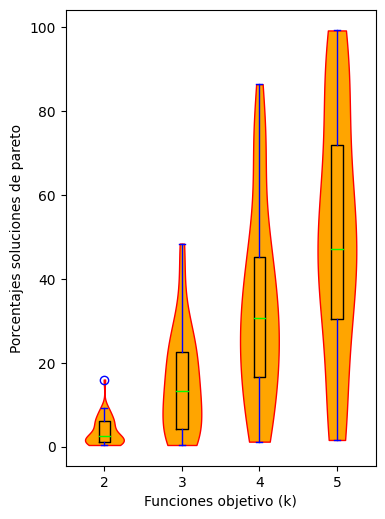
\includegraphics[width=\linewidth]{imagenes/p11p_violin.png}
\end{subfigure}
\caption{Gráfica de tiempo de ejecución.}
\label{fig:westminster}
\end{figure}
%%%%%%%%%%%%%%%%%%%%%%%  final 






\newpage
\section{Reto 1}
El primer reto es seleccionar un subconjunto (cuyo tamaño como un porcentaje del frente original se proporciona como un parámetro) del frente de Pareto de tal forma que la selección esté diversificada, es decir, que no estén agrupados juntos en una sola zona del frente las soluciones seleccionadas. Graficar los resultados de la selección, indicando con un color cuáles se incluyen en el subconjunto diverso.



%%%%%%%%%%%%%%%%%%%%% imagen 1
\begin{figure}[H]
\centering
\begin{subfigure}[b]{1.0\linewidth}
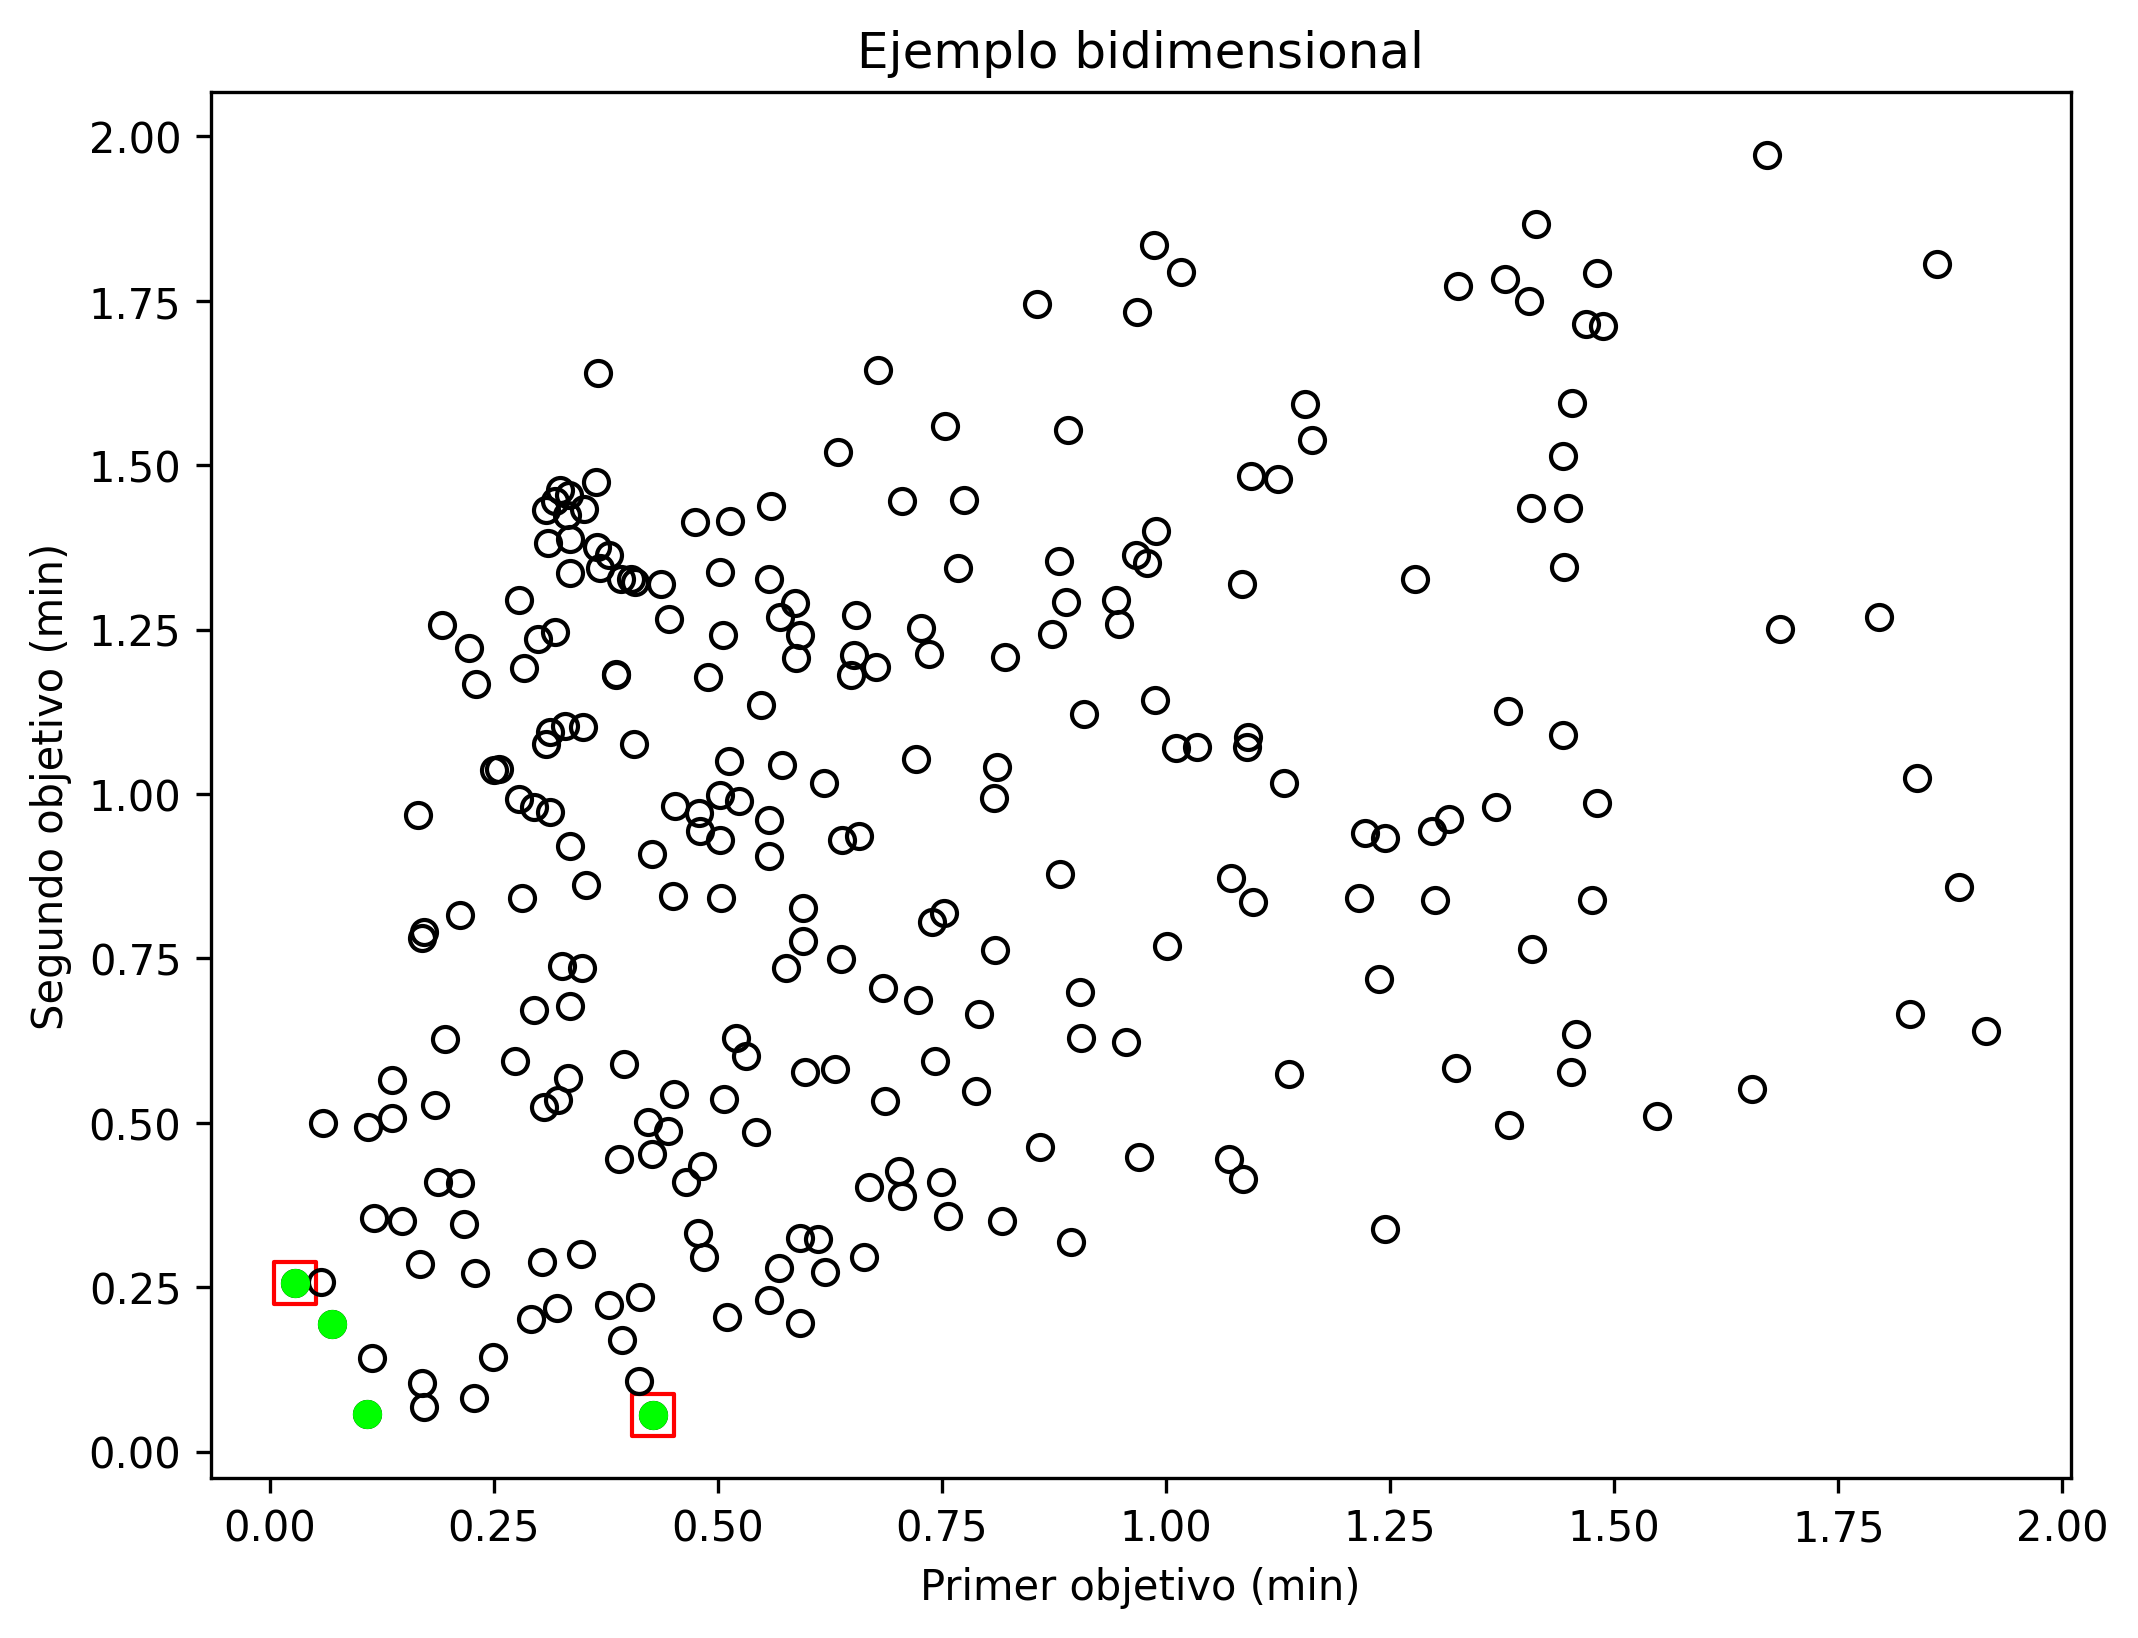
\includegraphics[width=\linewidth]{imagenes/Reto1_1.png}
\end{subfigure}
\caption{Gráfica de comportamiento regla 1.}
\label{fig:westminster}
\end{figure}
%%%%%%%%%%%%%%%%%%%%%%%  final 


%%%%%%%%%%%%%%%%%%%%% imagen 2
\begin{figure}[H]
\centering
\begin{subfigure}[b]{1.0\linewidth}
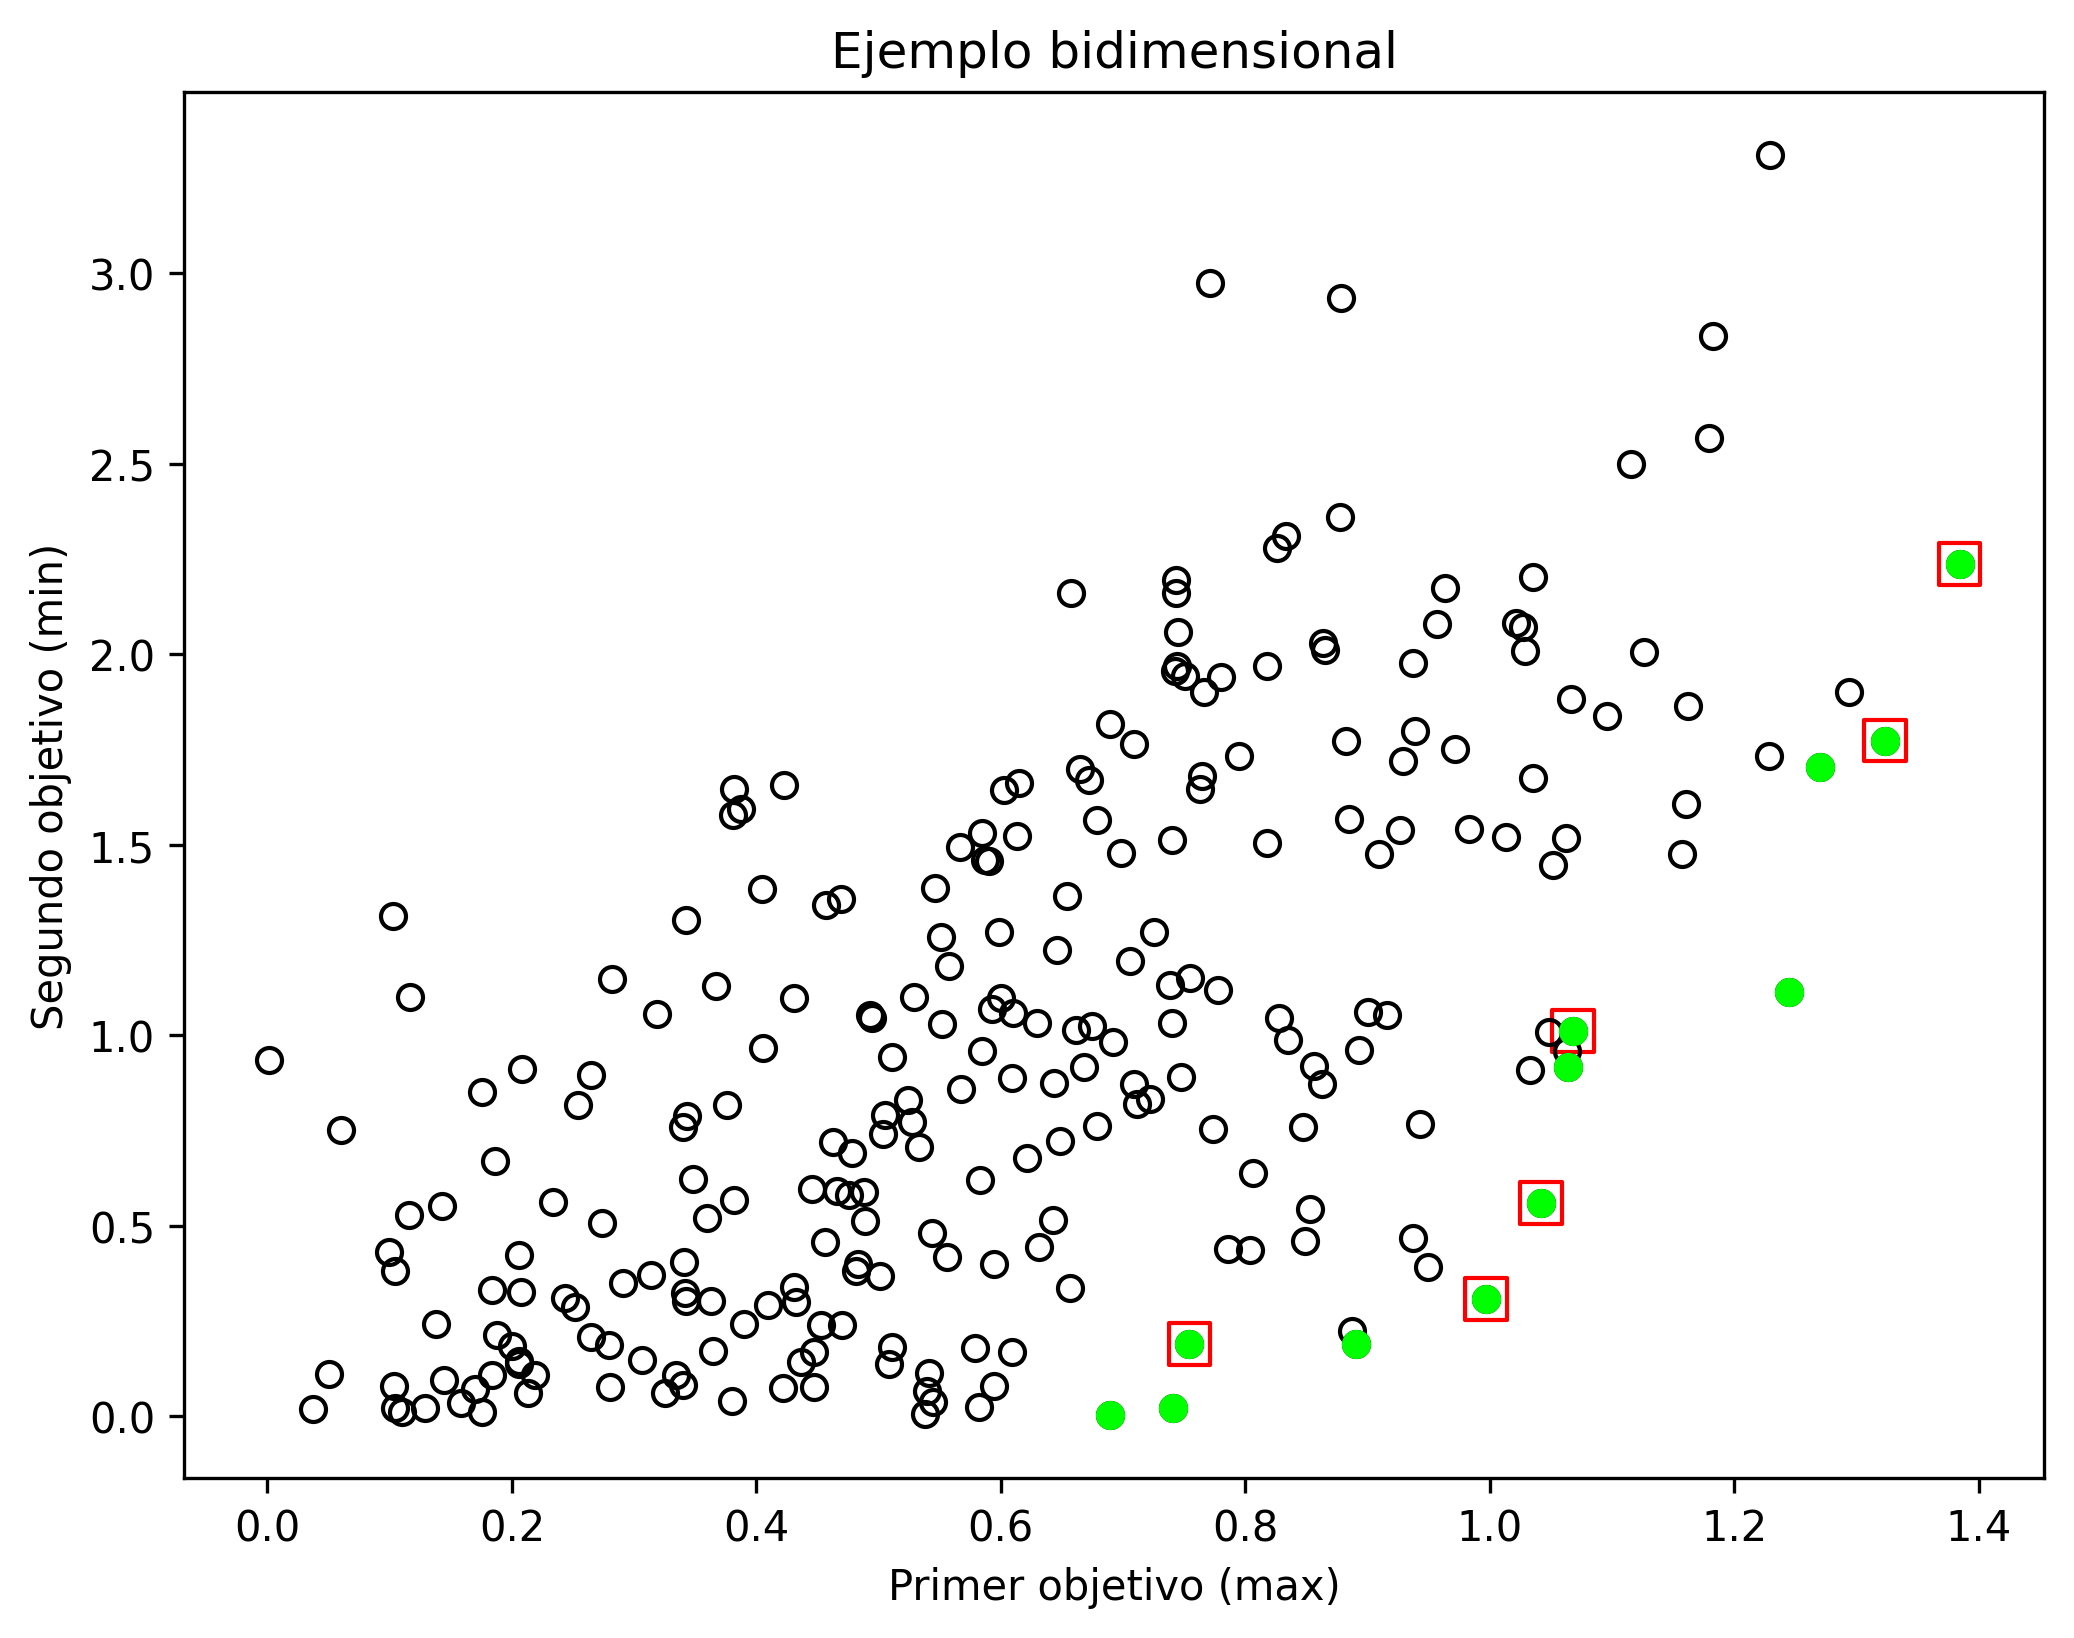
\includegraphics[width=\linewidth]{imagenes/Reto1_2.png}
\end{subfigure}
\caption{Grafica de comportamiento regla 2 .}
\label{fig:westminster}
\end{figure}
%%%%%%%%%%%%%%%%%%%%%%%  final 



%%%%%%%%%%%%%%%%%%%%% imagen 3
\begin{figure}[H]
\centering
\begin{subfigure}[b]{1.0\linewidth}
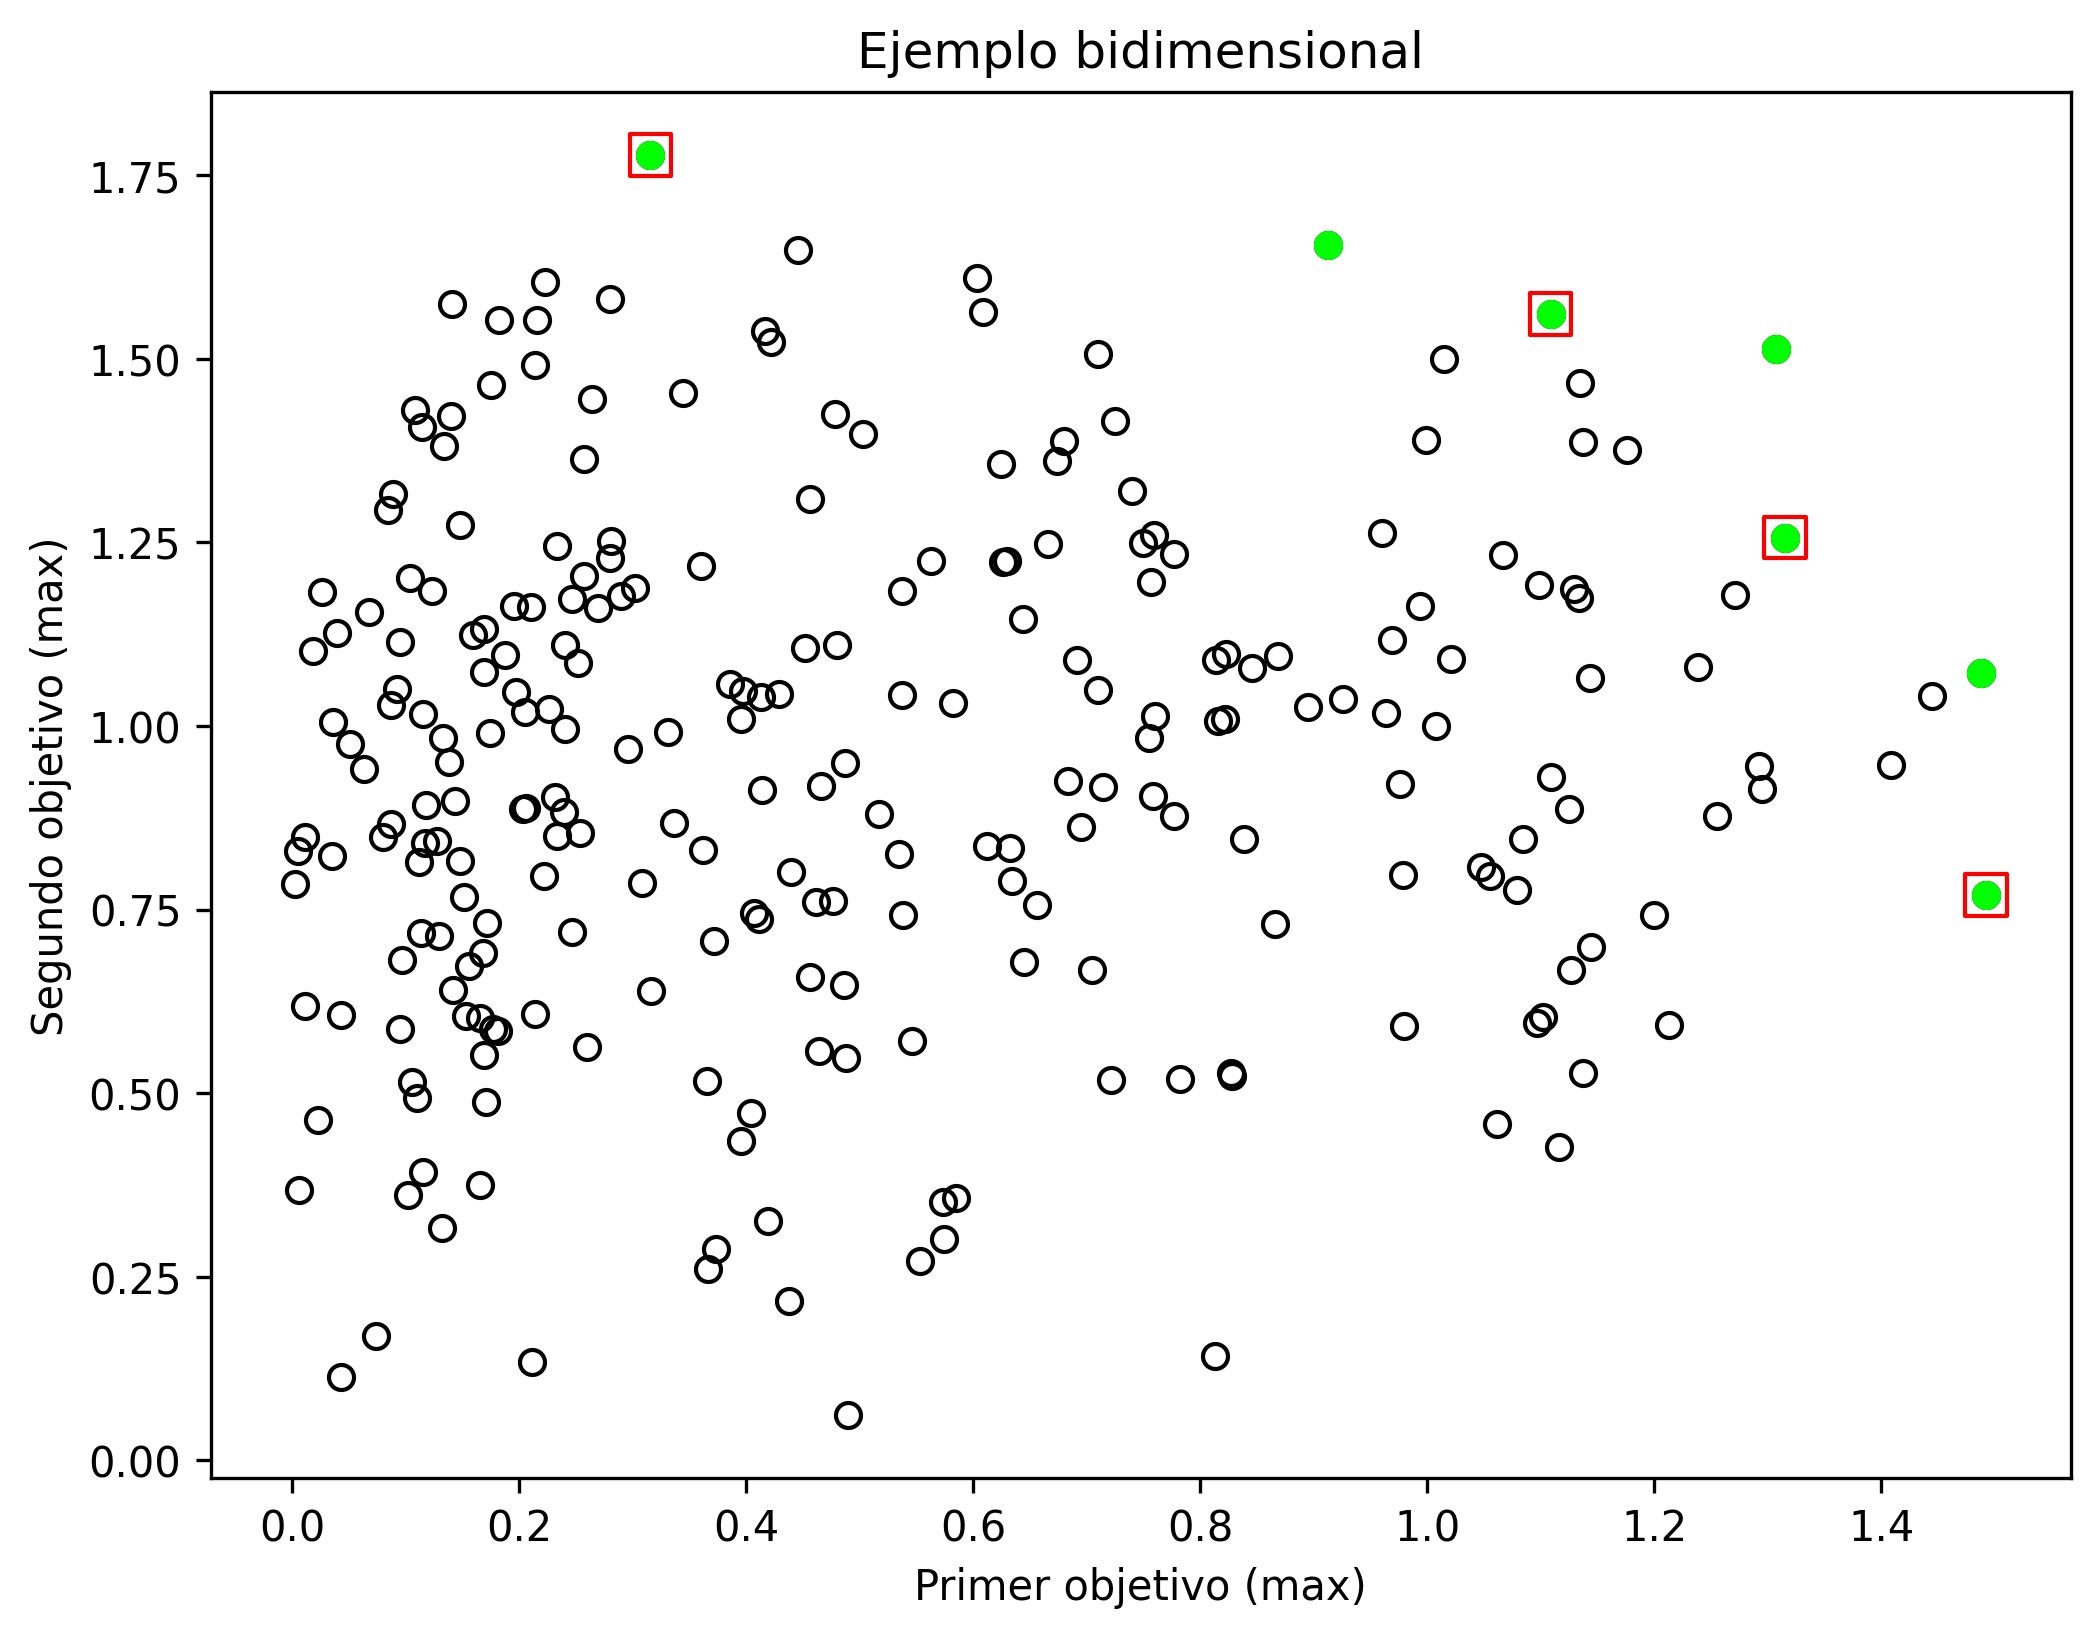
\includegraphics[width=\linewidth]{imagenes/Reto1_3.png}
\end{subfigure}
\caption{Grafica de comportamiento regla 3.}
\label{fig:westminster}
\end{figure}
%%%%%%%%%%%%%%%%%%%%%%%  final 
%%%%%%%%%%%%%%%%%%%%% imagen 4
\begin{figure}[H]
\centering
\begin{subfigure}[b]{1.0\linewidth}
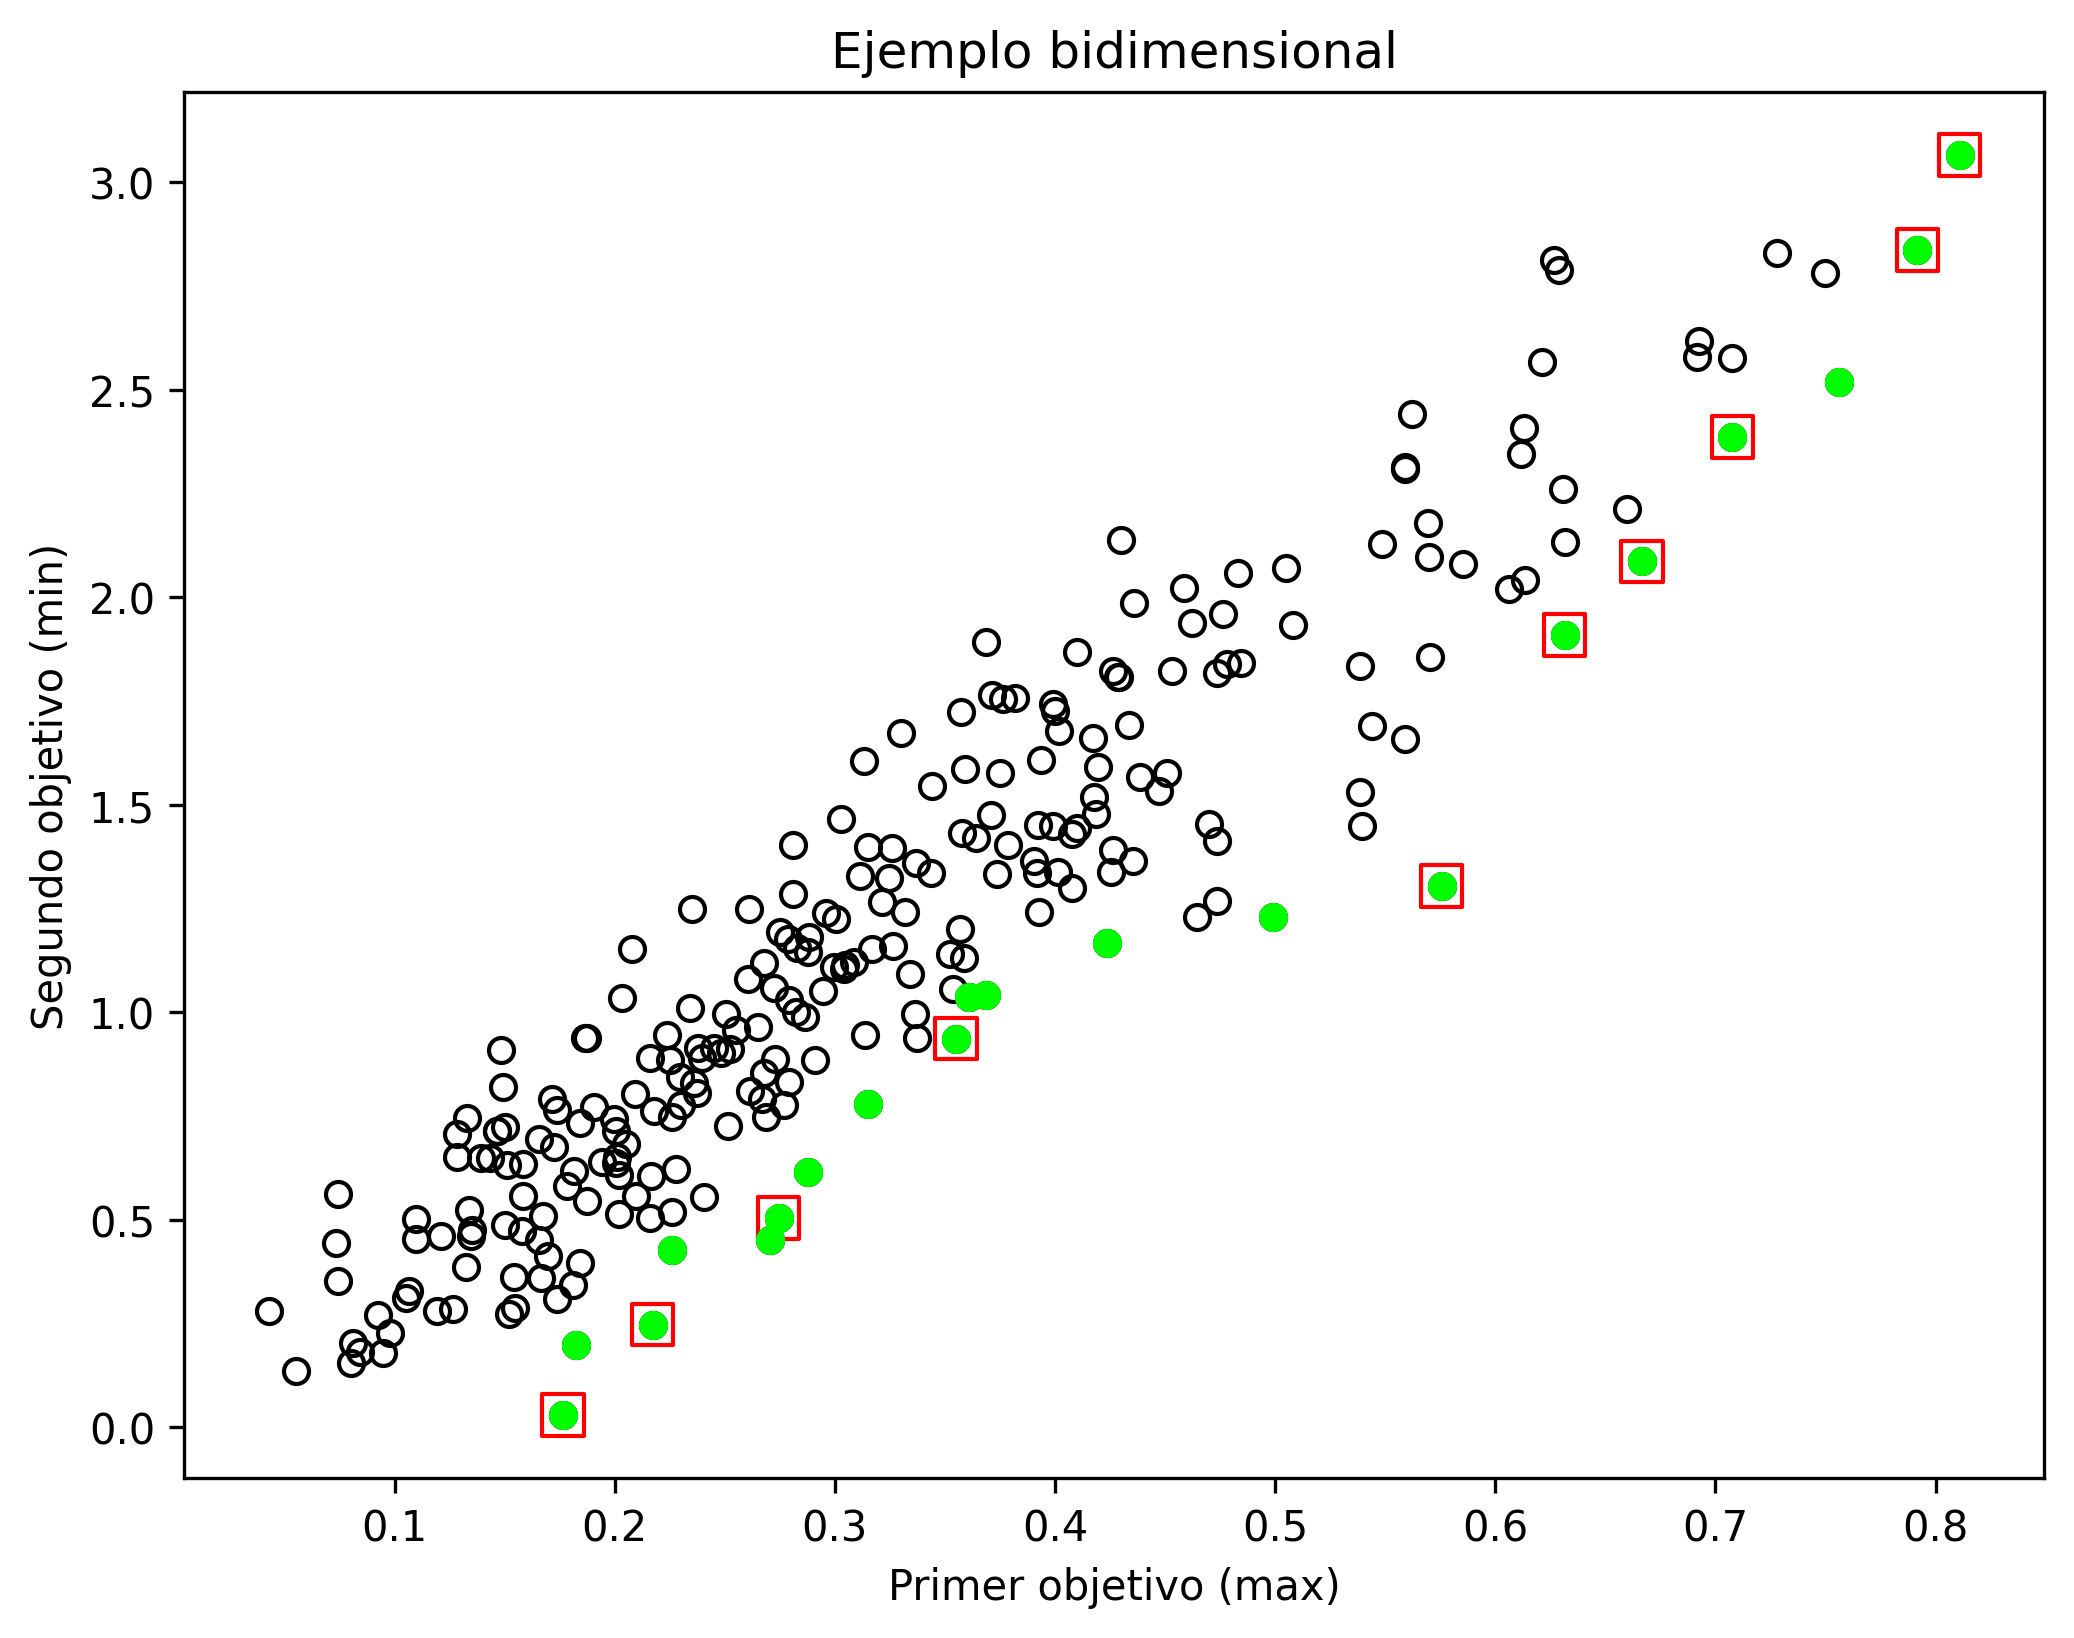
\includegraphics[width=\linewidth]{imagenes/Reto1_4.png}
\end{subfigure}
\caption{Gráfica de tiempo de ejecución.}
\label{fig:westminster}
\end{figure}
%%%%%%%%%%%%%%%%%%%%%%%  final 





 \section{Conclusión}
Se mostró con graficas de violín como va comportamiento del valor del objetivo al aumentar el valor, en el reto 1 calculando la distancia euclidiana podemos encerrar en círculos los más separados del resto de la pared de pareto.  

 \bibliography{bib.bib}
 \bibliographystyle{unsrtnat}

 \end{document}


